\documentclass[11pt,letterpaper]{article}
\usepackage[T1]{fontenc}
\usepackage[utf8]{inputenc}
\usepackage[margin=.88in,headheight=15pt]{geometry}
\usepackage{amsmath,amsthm,mathtools}
\usepackage{newtxtext,newtxmath,microtype}
\usepackage{booktabs,tabularx,array,longtable,enumitem,xcolor,tikz,fancyhdr,titlesec,needspace}
\usepackage{fontawesome5,xurl,hyperref,placeins,listings}
\usetikzlibrary{arrows.meta,positioning,calc,fit}
\definecolor{ink}{HTML}{302045}
\definecolor{accent}{HTML}{7252A3}
\definecolor{gold}{HTML}{AD8037}
\definecolor{pale}{HTML}{F5F2FA}
\definecolor{muted}{HTML}{665E70}
\hypersetup{colorlinks=true,linkcolor=accent,citecolor=accent,urlcolor=accent,
 pdftitle={Autonomous Enterprises: Activate. Evolve. Scale.},pdfauthor={Vincent Boucher},
 pdfsubject={Reusable launch kits and rejection-only improvement transfer}}
\urlstyle{same}
\pagestyle{fancy}\fancyhf{}
\fancyhead[L]{\footnotesize\sffamily AUTONOMOUS ENTERPRISES}
\fancyhead[R]{\footnotesize\sffamily MONTREAL.AI / QUEBEC.AI}
\fancyfoot[C]{\thepage}\renewcommand{\headrulewidth}{.3pt}
\setlength{\parskip}{.23em}\setlength{\parindent}{1em}\setlength{\emergencystretch}{2em}
\renewcommand{\arraystretch}{1.15}
\setlist{nosep,leftmargin=1.3em}
\titleformat{\section}{\large\bfseries\color{ink}}{\thesection}{.65em}{}
\titleformat{\subsection}{\normalsize\bfseries\color{ink}}{\thesubsection}{.6em}{}
\titlespacing*{\section}{0pt}{1.2em}{.55em}
\titlespacing*{\subsection}{0pt}{.85em}{.35em}
\newcolumntype{Y}{>{\raggedright\arraybackslash}X}
\newcolumntype{P}[1]{>{\raggedright\arraybackslash}p{#1}}
\newcommand{\Om}{SUCCESSOR~$\Omega$}
\newcommand{\insight}[1]{\begin{center}\setlength{\fboxsep}{9pt}\fcolorbox{accent}{pale}{\begin{minipage}{.92\linewidth}#1\end{minipage}}\end{center}}
\newtheorem{proposition}{Proposition}[section]
\newtheorem{theorem}[proposition]{Theorem}
\newtheorem{corollary}[proposition]{Corollary}
\lstset{basicstyle=\small\ttfamily,breaklines=true,columns=fullflexible,keepspaces=true,frame=single,rulecolor=\color{accent!40},showstringspaces=false}
\renewcommand{\topfraction}{.95}\renewcommand{\bottomfraction}{.85}\renewcommand{\textfraction}{.05}\renewcommand{\floatpagefraction}{.8}
\pdfinfoomitdate=1\pdftrailerid{}
\begin{document}
\thispagestyle{plain}
\begin{center}
{\small\sffamily\color{accent} MONTREAL.AI\quad /\quad TRANSFORMATIONAL INTELLIGENCE $\infty$}\par
\vspace{.65em}
{\Large\color{accent}\faStar\quad\faCogs}\par
\vspace{.6em}
{\fontsize{26}{30}\selectfont\bfseries\color{ink} AUTONOMOUS ENTERPRISES}\par
\vspace{.4em}
{\fontsize{23}{27}\selectfont\bfseries\color{accent} ACTIVATE. EVOLVE. SCALE.}\par
\vspace{.65em}
{\large Reusable Launch Kits with Rejection-Only Improvement Transfer}\par
\vspace{.9em}
{\large Vincent Boucher}\par
MONTREAL.AI\;\textbullet\;QUEBEC.AI\par
Montr\'eal, Qu\'ebec, Canada\par
\vspace{.4em}
22 October 2026\quad\textbullet\quad Research manuscript and runnable local companion
\end{center}
\begin{abstract}
A useful enterprise should not wait for its improvement machinery to become extraordinary before it can begin. We construct a small launch kit that starts with available deterministic tools, executes an explicit mission, checks the actual output, and retains a bounded way to improve the next launch. Three materially different local offerings---range analytics, polynomial composition, and dependency reachability---share one operating path without sharing budgets or authority. The central mechanism transfers \emph{rejection experience}, not acceptance: an evidence-derived test prefix can expose defective improvement candidates earlier, but every surviving candidate still faces the complete unchanged acceptance suite. We prove preservation of that finite acceptance predicate and a tight bound on additional screening work after an unfavorable task shift. The reference activates all three offerings and delivers independently checked results. A schedule learned on range analytics reduces next-cycle candidate checks from 223 to 118 for polynomial composition and from 233 to 89 for reachability. Charging its 90-check source qualification leaves 159 fewer checks across those two continuations; log processing and human engineering remain separate costs. A strong conventional ordering wins the polynomial comparison, and a second learned update is rejected because it worsens the next cycle. A 24-job workload runs with one, two and four workers; four are slower than two in the recorded run. The contribution is an executable organizational synthesis with bounded transfer, failures and a deployment handoff, not a new test-prioritization algorithm, demonstrated general recursive self-improvement, or three paying businesses.
\end{abstract}
\insight{\centering\textbf{Launch the useful version. Improve the machinery.}\par\smallskip
Share what helps the next enterprise---not yesterday's authority.}
\begin{center}\small
\textbf{Find your Alpha. Build your SUCCESSOR $\Omega$.}\par
\href{https://github.com/MontrealAI/AGI-Alpha-Agent-v0}{github.com/MontrealAI/AGI-Alpha-Agent-v0}
\end{center}
\clearpage

\section{Build the means to begin}
A research team needs exact summaries of many intervals in a public time series. A second team needs to combine two discrete models. A software maintainer needs to know which components are reachable through a dependency graph. These are different useful outcomes. None requires a new foundation model, a token launch, a simulated economy, or a committee of agents before a first local delivery can be checked.

What each does need is a short path from intention to accountable execution: a precise input, a qualified implementation, a resource allowance, an acceptance procedure and an inspectable result. The opportunity studied here is to make that path reusable, and then make the mechanism that improves it reusable too. The first product is useful computation. The next retained asset is a less wasteful way of qualifying a different product's improvement.

\insight{\textbf{Do not make the future enterprise a prerequisite for the first useful enterprise.}\par\smallskip
Activate from what works now. Let operating evidence identify the next worthwhile construction.}

The immediate predecessor, \emph{Build the Means of Building}, made productive inheritance concrete: one generated operator changed the work needed to qualify another, and a capital--capability law priced the consequence of losing that inheritance \cite{predecessor}. It did not establish a reusable launch process for distinct offerings or an empirically improving launch mechanism. This paper does not transplant its operation counts into a new claim. It changes the unit of construction from an arithmetic foundry to a \emph{launch kit with an evidence-derived improvement procedure}.

The change is modest enough to ship. A standard-library Python command activates a mission, runs a reviewed local kernel, checks its complete requested output against a separate defining implementation, and records the result. A distinct variant changes the mission and input, not the platform. An optional improvement cycle tests alternatives; a learned ordering can make later cycles cheaper without changing which alternatives qualify. The baseline remains available throughout.

The scientific claim is correspondingly specific. This is an architectural synthesis and an executed operational experiment, not a new universal optimizer. Test prioritization, counterexample-guided synthesis, versioned workflows and transactional accounting have substantial predecessors \cite{rothermel,elbaum,cegis,sqlite}. Our contribution is their small, bounded integration around \emph{cross-offering improvement transfer}, with a sharp screening-overhead limit, actual launch/recovery tests and explicit rejection of an unsuccessful second update.

\subsection{Three boundaries before three verbs}
A runnable demonstration is not an externally deployed service. A deployed service is not a paying enterprise. A paying enterprise is not evidence of indefinite profitable expansion. The companion reaches the first category: three functioning local offering instances and their operating evidence. There is no customer, price acceptance, invoice or payment in the experiment.

Likewise, a better task implementation, reuse of an artifact, and improvement of the mechanism that produces later improvements are distinct. We measure a bounded example of the third: earlier failure records alter a later candidate-evaluation procedure. The update family is human-authored and finite; no model weights, self-generated learning algorithm or autonomous discovery of a new primitive are involved.

\section{One architecture; a thin operating path}
\textbf{AGI ALPHA organizes intelligence.} It connects tools, agents, memory, work and validation. Its architectural manuscript proposes an organizational substrate and an Evidence Docket discipline, not an already validated general enterprise \cite{alpha}. \textbf{Transformational Intelligence $\infty$ changes the game.} It distinguishes the intended purpose from an inherited formulation and its evaluator \cite{ti}. Here, the removable assumption is that each new offering must reconstruct its launch and improvement procedure from scratch. The preserved obligations are the requested mathematics, input scope, current permission and acceptance tests.

The six stages remain logical responsibilities, not six compulsory model calls. \textbf{Out-Learn} retains observed failures; \textbf{Out-Think} separates mission state from shared knowledge; \textbf{Out-Design} constructs an executable service configuration; \textbf{Out-Strategise} chooses an evaluation order and retains the baseline; \textbf{Out-Execute} delivers a checked result; \textbf{Out-Evolve} tests and versions a change to the next improvement cycle. The three-verb lifecycle is their operating realization, not a seventh Out-stage.

\begin{figure}[htbp]\centering
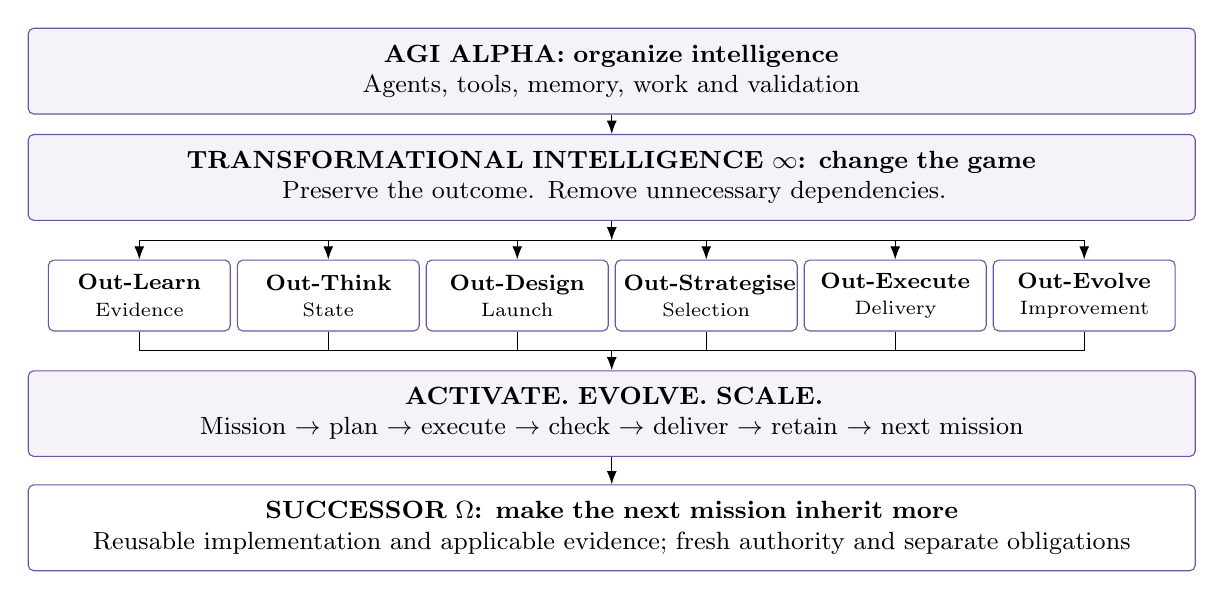
\begin{tikzpicture}[font=\small,>=Latex,
 b/.style={draw=accent,rounded corners=2pt,align=center,inner sep=6pt}]
\node[b,fill=pale,text width=14.4cm] (a) at (0,0) {\textbf{AGI ALPHA: organize intelligence}\par Agents, tools, memory, work and validation};
\node[b,fill=pale,text width=14.4cm] (t) at (0,-1.35) {\textbf{TRANSFORMATIONAL INTELLIGENCE $\infty$: change the game}\par Preserve the outcome. Remove unnecessary dependencies.};
\draw[->] (a)--(t);
\foreach \id/\x/\title/\sub in {1/-6/Out-Learn/Evidence,2/-3.6/Out-Think/State,3/-1.2/Out-Design/Launch,4/1.2/Out-Strategise/Selection,5/3.6/Out-Execute/Delivery,6/6/Out-Evolve/Improvement}{
\node[b,text width=2.1cm,inner sep=3pt,font=\footnotesize,minimum height=.9cm] (s\id) at (\x,-2.85) {\textbf{\mbox{\title}}\par\scriptsize\sub};}
\draw[->] (t.south)--(0,-2.15);
\draw (-6,-2.15)--(6,-2.15);
\foreach \id in {1,...,6}{\draw[->] (s\id.north |- 0,-2.15)--(s\id.north);}
\node[b,fill=pale,text width=14.4cm] (l) at (0,-4.35) {\textbf{ACTIVATE. EVOLVE. SCALE.}\par Mission $\to$ plan $\to$ execute $\to$ check $\to$ deliver $\to$ retain $\to$ next mission};
\draw (-6,-3.55)--(6,-3.55);
\foreach \id in {1,...,6}{\draw (s\id.south)--(s\id.south |- 0,-3.55);}
\draw[->] (0,-3.55)--(l.north);
\node[b,text width=14.4cm] (o) at (0,-5.8) {\textbf{SUCCESSOR $\Omega$: make the next mission inherit more}\par Reusable implementation and applicable evidence; fresh authority and separate obligations};
\draw[->] (l)--(o);
\end{tikzpicture}
\caption{The hierarchy realized as data and executable transitions. The local companion implements the narrow service, checking and improvement path. Model orchestration, commissioned work and settlement are optional integration surfaces, not executed claims.}
\label{fig:architecture}
\end{figure}

\subsection{What crosses a boundary}
A mission contains its identifier, family, data, acceptance rule, local resource ceiling and explicit local-computation authority. Activation binds it to the current source identity. The operating state contains the mission, implementation version, charged/reserved work, attempt states and permission. Shared state contains only reviewed service code and a versioned rejection-order profile. A profile contains no key, spending grant, payment claim or previously accepted customer output.

The delivery record contains the actual input and output, current code identity, execution/checking work, attempt identifier, technical match and current authorization result. Commercial acceptance is explicitly false and receipts are null. A technical failure remains a rejection; a budget interruption remains incomplete work. These states are useful engineering outcomes, not alternative ways to declare a successful enterprise.

\section{Activate three useful variants now}
The launch kit uses Python's standard library: exact integer arithmetic, queues, JSON, SQLite and bounded local processes. There is no paid API, provider key, model download, blockchain call or browser dependency. That is not a rejection of capable models: it is the smallest construction for these missions. A reviewed model-generated candidate can be added later under a separately qualified execution interface; this companion does not execute arbitrary generated code.

\begin{table}[htbp]\centering\small
\caption{Six plain answers for each proposed offering. Beneficiaries and prices are hypotheses, not observed customers or quotations.}
\begin{tabularx}{\linewidth}{@{}P{2.2cm}YYY@{}}\toprule
& Range analytics & Polynomial composition & Dependency reachability\\\midrule
Who benefits? & Researchers analysing public integer series & Scientific-software teams combining discrete models & Maintainers inspecting public dependency graphs\\
Outcome & Exact sums for requested half-open intervals & Full coefficient vector of a polynomial product & Reachable nodes for each supplied source\\
Proof of delivery & Separate direct summation on the actual request & Independent coefficient-by-coefficient product & Independent transitive-closure calculation\\
Tools now & Prefix sums or direct sums; Python & Sparse or dense multiplication; Python & Queue traversal or fixed-point search; Python\\
Delivery cost & Recorded work and elapsed time; human semantic review unmeasured & Same accounting; review and support unmeasured & Same accounting; graph interpretation unmeasured\\
Next deployment & One independently selected public-series report & One external numerical-reproduction request & One public repository's reviewed graph export\\\bottomrule
\end{tabularx}
\label{tab:offers}
\end{table}

A bounded report, its exact inputs, its check and a fixed-price proposal are sufficient to begin a commercial conversation. As deliberately unoffered price hypotheses, consider US\$150, US\$250 and US\$200 respectively for one scoped report plus review. These values are author-selected discovery prompts, not evidence of willingness to pay, viable margins or market pricing. Basic implementations are freely available elsewhere; a paid service would need to justify its data mapping, reproducibility, interpretation, adaptation and support. A beneficiary who can use the local command directly may rationally pay nothing.

The implementation supports integer inputs only, with explicit size limits. It does not interpret arbitrary CSV semantics, discover a repository graph automatically, certify a probabilistic model's assumptions, or infer a customer objective. The supplied examples are authored representative tasks. A first externally useful engagement needs an actual dataset, an agreed interpretation and actual acceptance, but not a new platform.

\subsection{From an inert mission to an accepted local result}
Activation validates identifiers, types, dimensions, budget and permission, then persists the mission. Before execution, one SQLite transaction reserves a conservative work allowance from that mission alone. A separate defining implementation checks the requested output. Acceptance is committed only after the current permission is re-read. Unused reserved work is released; a failed or interrupted attempt is not erased. A content-bound prior accepted result can be reopened without another debit, while a new operation still requires current authority.

The work unit is an explicit counter increment in the service or reference implementation, not a processor instruction or currency. The conservative reservation also bounds the size-limited local workload. The improvement loop has a separately supplied per-call test allowance, recorded as candidate evaluations; those units are not silently added to arithmetic work or money.

The initial qualified baseline runs before tuning. All three examples produce accepted local outputs. The observed configuration writes took 5.59, 2.96 and 2.66 milliseconds for the range, polynomial and graph examples respectively. These single local measurements exclude creating the templates, interpreting a customer request and reviewing a delivery; they are not time-to-business estimates. Tuning subsequently finds the already available conventional implementation with lower counted execution work, when one exists; a zero-query range mission retains its baseline because building a prefix array would add useless work. This control matters: evolution is permitted to decide not to change.

\Needspace{7\baselineskip}
\section{Evolve the improver without weakening acceptance}
\subsection{The bottleneck exposed by operation}
The improvement laboratory has seven reviewed candidate identifiers per family: five intentionally defective fixtures, a correct baseline and a conventional optimized implementation. The defects exercise empty inputs, boundary semantics, duplicates, signs/directions and structure. They are authored faults, not measured model-error frequencies. The production launcher refuses these fault identifiers.

Each candidate is checked against 39 cases: 24 ordinary generated cases and fifteen explicit edge cases. In the initial ordering, several bad candidates pass the ordinary block before failing an edge case. Repeating that validation itinerary on every new offering wastes candidate evaluations. The transformation is not to remove tests. It is to retain what earlier failures teach about \emph{which tests should be tried first}.

A small learner counts observed failures and exposures by test group, ranks groups by their observed failure/exposure ratio, and proposes a prefix with at most one early representative per selected group. The retained prefix is followed by every remaining test in its original order, without duplication. A failing candidate stops early. A surviving candidate must finish the entire unchanged suite. Previous output values and acceptance decisions do not transfer; the new offering computes its own reference answers.

The source range campaign selects four representatives, in the group order structure, empty, negative and duplicates. Labels are suite-local routing hints: for example, the reachability suite maps direction-sensitive examples to its designated group. This is a disclosed mapping, not a learned universal ontology. A misleading mapping may waste work, but cannot make a failing full predicate pass.

\begin{figure}[htbp]\centering
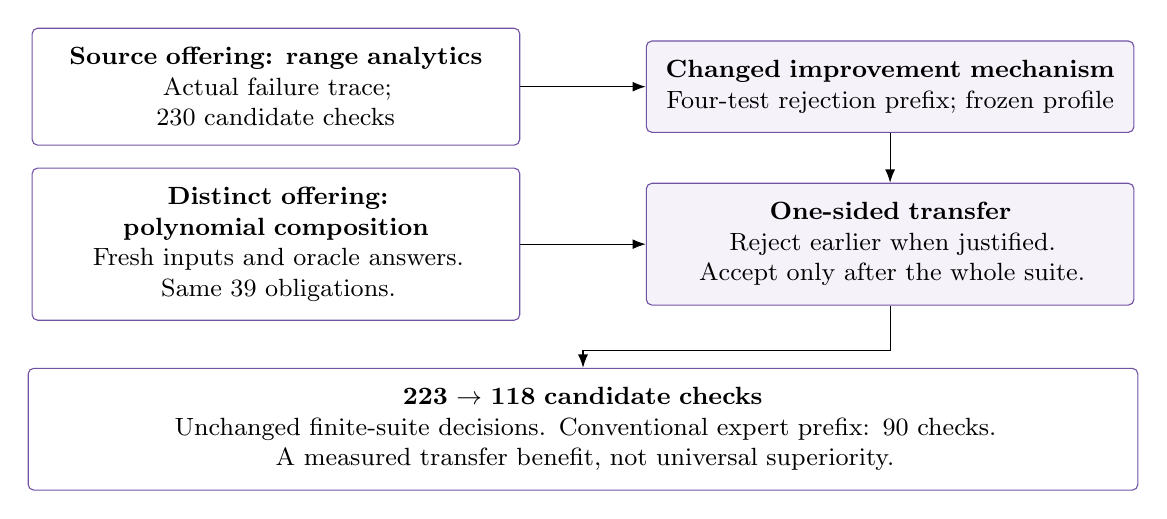
\begin{tikzpicture}[font=\small,>=Latex,
 b/.style={draw=accent,rounded corners=2pt,align=center,inner sep=7pt}]
\node[b,text width=5.7cm] (old) at (-3.9,0) {\textbf{Source offering: range analytics}\par Actual failure trace; 230 candidate checks};
\node[b,fill=pale,text width=5.7cm] (learn) at (3.9,0) {\textbf{Changed improvement mechanism}\par Four-test rejection prefix; frozen profile};
\draw[->] (old)--(learn);
\node[b,text width=5.7cm] (next) at (-3.9,-2) {\textbf{Distinct offering:}\par\textbf{\mbox{polynomial composition}}\par Fresh inputs and oracle answers.\par Same 39 obligations.};
\node[b,fill=pale,text width=5.7cm] (check) at (3.9,-2) {\textbf{One-sided transfer}\par Reject earlier when justified.\par Accept only after the whole suite.};
\draw[->] (learn)--(check);\draw[->] (next)--(check);
\node[b,text width=13.6cm] (result) at (0,-4.35) {\textbf{223 $\to$ 118 candidate checks}\par Unchanged finite-suite decisions. Conventional expert prefix: 90 checks.\par A measured transfer benefit, not universal superiority.};
\draw[->] (check.south)--(3.9,-3.35)--(0,-3.35)--(result.north);
\end{tikzpicture}
\caption{The actual causal transfer: the next evaluation invokes the frozen source-derived ordering. Removing that ordering restores the fixed baseline. The known-good task implementation remains available while improvement is tested.}
\label{fig:transfer}
\end{figure}

\subsection{The narrow guarantee that permits transfer}
Let $T=(t_1,\ldots,t_n)$ be deterministic, side-effect-free predicates on a fixed candidate $c$. Acceptance is
\begin{equation}
 A(c)=\bigwedge_{i=1}^{n}t_i(c).
\end{equation}
A prefix $P$ is an ordered list of $k$ distinct members of $T$. The transformed schedule is $P$ followed by $T\setminus P$ in its original order. Test outcomes must not depend on evaluation order; the candidate, inputs and predicate implementations stay fixed.

\Needspace{16\baselineskip}
\begin{theorem}[Rejection-only inheritance]
The transformed schedule preserves $A(c)$. Suppose each test has a fixed nonnegative evaluation cost $w_i(c)$ for that candidate. If both procedures stop at their first failure or after the full suite, then
\begin{equation}
 C_P(c)\le C_T(c)+\sum_{t_i\in P}w_i(c).
 \label{eq:bound}
\end{equation}
If $c$ passes, $C_P(c)=C_T(c)=\sum_iw_i(c)$. With unit test costs, the worst additional number of checks is at most $k$; for $0\le k<n$, this bound is attainable.
\end{theorem}
\begin{proof}
Every predicate occurs once, so the conjunction is unchanged. If a prefix test fails, the transformed procedure pays no more than the prefix sum. Otherwise it proceeds through the residual original order. Its first residual failure is no later than the original first failing predicate after prefix members have been removed. Its paid tests therefore lie in the union of the original paid prefix and $P$, giving (\ref{eq:bound}). A passing candidate runs every predicate once. For sharpness, make only $t_1$ fail and choose $k$ later passing predicates for $P$: the original cost is one and the transformed cost is $k+1$.
\end{proof}

This is an elementary scheduling guarantee, not a newly invented theory of testing. Its organizational role is important: shared experience can alter the itinerary without acquiring authority to change the destination. Under a finite allowance, exhaustion yields \texttt{INCOMPLETE}, never acceptance. Reordering can change which failing candidate finishes within that allowance. It cannot license a partial pass. Scheduling, hashing, log-reading and profile-construction overhead remain additional to the predicate costs.

The conditions are real. Stateful tests, candidate mutation, stochastic replies without a controlled coupling, timeouts interpreted as passes, or an omitted predicate can invalidate the equivalence. A changed evaluator needs its own review. Content identities detect changed bytes but do not establish that the predicates reflect a beneficiary's needs.

\subsection{What is, and is not, recursive}
The source-derived prefix changes the \emph{process that evaluates later implementation improvements}. Its next use is therefore a measured meta-level adaptation, not merely retrieval of a previous answer. The learner that constructs such prefixes remains fixed and human-authored. We use ``bounded improvement of the improver'' for the demonstrated mechanism; we do not infer general recursive self-improvement, autonomous discovery of a learning algorithm or gains in model weights.

A second update is built from the source and first transfer trace, frozen before evaluating the next graph cycle. It takes 90 checks where the retained first update takes 89, with the same decisions. The study rejects it. This negative result is central: a system that promotes every new version would confuse change with progress.

\section{Evidence: improvements, ties and losses}
\subsection{The matched next-cycle comparison}
All comparison methods use the same candidate set, actual inputs, defining reference answers and 39 acceptance predicates. The treatment changes only test order. Fixed order is the no-inheritance baseline. Move-to-front is a conventional within-campaign adaptive method that moves the last failing group to the front. An expert prefix selects one edge case from each of five groups without learning. It is a strong same-capability alternative, not a weakened competitor.

\begin{table}[htbp]\centering\small
\caption{Candidate evaluations on the two continuation offerings. Lower is better; the same baseline and optimized candidate pass in every column. These are authored defect experiments, not frontier-model benchmark scores.}
\begin{tabularx}{\linewidth}{@{}Yrrrr@{}}\toprule
Offering & Fixed & Learned prefix & Move-to-front & Expert prefix\\\midrule
Polynomial composition & 223 & 118 & 172 & \textbf{90}\\
Dependency reachability & 233 & \textbf{89} & 233 & 93\\\bottomrule
\end{tabularx}
\label{tab:transfer}
\end{table}

The source campaign costs 230 checks. Testing the proposed schedule on that source adds 90 checks. Across the two continuations, the learned schedule avoids $105+144=249$ checks relative to fixed order; charging the 90-check source qualification leaves 159 fewer candidate evaluations. Equivalently, the three-cycle fixed path uses $230+223+233=686$ checks, while the learned path including its qualification uses $230+90+118+89=527$. These totals do not convert test counts into currency or imply that the learned method beats the expert: the expert is materially better on polynomial composition.

Profile formation also scans 230 saved observations and sorts six group scores. Those operations are recorded separately rather than declared free or numerically interchangeable with executing a candidate. Human research, code authoring and review are unmetered. An end-to-end cost comparison must price those terms. For this experiment, the measurable claim is fewer candidate evaluations after the stated qualification charge, not a complete commercial saving.

A fresh confirmation block uses 24 additional ordinary-case seeds across the two continuation families. The edge-case fixtures and candidate defects remain the same authored taxonomy; these are implementation checks, not 24 independent discoveries or a representative market sample. All finite-suite decisions remain equal. A complete truth-vector check covers 2,528 small configurations of prefix length, original order and failure pattern, confirming the screening bound in those finite instances; the theorem establishes its general conditional statement.

\subsection{The baseline can win}
The unfavorable-shift control makes the first ordinary predicate the only failure. The four inherited prefix tests now increase rejection work from one check to five, attaining the bound. If all predicates pass, both orders run 39 checks. The learned ordering therefore cannot create a uniform efficiency gain. It earns use through observed or defensibly expected failure structure, not the name ``evolution.''

The implementation also refuses to adopt the optimized range kernel when a request has no queries: direct execution performs no summation while a prefix array would do unnecessary work. An optimization should pay for its construction, qualification and maintenance over a plausible reuse horizon. With improvement cost $H$ and expected per-use saving $s>0$ in one genuinely comparable unit, its narrow break-even condition is $Ns>H$. Unknown $H$, $s$, demand or maintenance remains unknown; the equation is not a sales forecast.

\subsection{Actual outputs and the cost of checking them}
The local lifecycle first delivers each baseline result, then runs its improvement campaign and delivers again using the selected conventional implementation. The mathematical purpose is unchanged. Independent reference checking is charged rather than omitted from the claimed benefit.

\begin{table}[htbp]\centering\small
\caption{Recorded work counters for the three example deliveries. The reference checker is unchanged. Work units are explicit source-level increments, not processor instructions, wall-clock time, energy or money.}
\begin{tabularx}{\linewidth}{@{}Yrrrr@{}}\toprule
Offering & Baseline execution & New execution & Checking & Total before $\to$ after\\\midrule
Range analytics & 4,740 & 276 & 4,740 & 9,480 $\to$ 5,016\\
Polynomial composition & 4,704 & 208 & 4,608 & 9,312 $\to$ 4,816\\
Dependency reachability & 209 & 40 & 5,832 & 6,041 $\to$ 5,872\\\bottomrule
\end{tabularx}
\label{tab:work}
\end{table}

The graph example illustrates a consequential bottleneck: execution improves, but validation dominates the total. Copying more executors or celebrating only kernel savings would obscure it. The two current-input implementations are also executed during selection, costing 5,016, 4,912 and 249 counter units respectively; those selection probes are additional recorded work, not silently included in one later delivery. The study separately reports candidate checks and source/profile overhead.

\section{Scale useful delivery, not instance count}
\subsection{A real bounded concurrency comparison}
A fixed workload contains 24 distinct input jobs: eight per offering. It is run on the same host with one, two and four worker processes. Every setting accepts all 24 requested outputs; the workload total is 9,870,487 declared execution-plus-checking increments in each setting. Inputs and correctness requirements are unchanged, while allocated process concurrency increases. This is not a matched-core efficiency experiment.

\begin{table}[htbp]\centering\small
\caption{One recorded local run per setting, including process startup and local persistence. Times are descriptive, not confidence intervals or a universal ordering. Python 3.13.5; Linux x86-64; five CPUs reported by the environment.}
\begin{tabular}{@{}rrrr@{}}\toprule
Workers & Accepted jobs & Elapsed seconds & Jobs/second\\\midrule
1 & 24 & 1.991 & 12.05\\
2 & 24 & 1.400 & 17.15\\
4 & 24 & 1.585 & 15.14\\\bottomrule
\end{tabular}
\label{tab:scale}
\end{table}

Four workers are slower than two in this run. The experiment does not isolate which combination of process startup, CPU scheduling, checking and serialized SQLite transactions causes that difference. It establishes a narrower useful point: increasing replica count did not deliver monotone observed throughput. Repeated workload-balanced runs on a deployment machine are needed before setting a production concurrency policy. Separate reruns retain their actual timings rather than byte-match nondeterministic time.

\begin{figure}[htbp]\centering
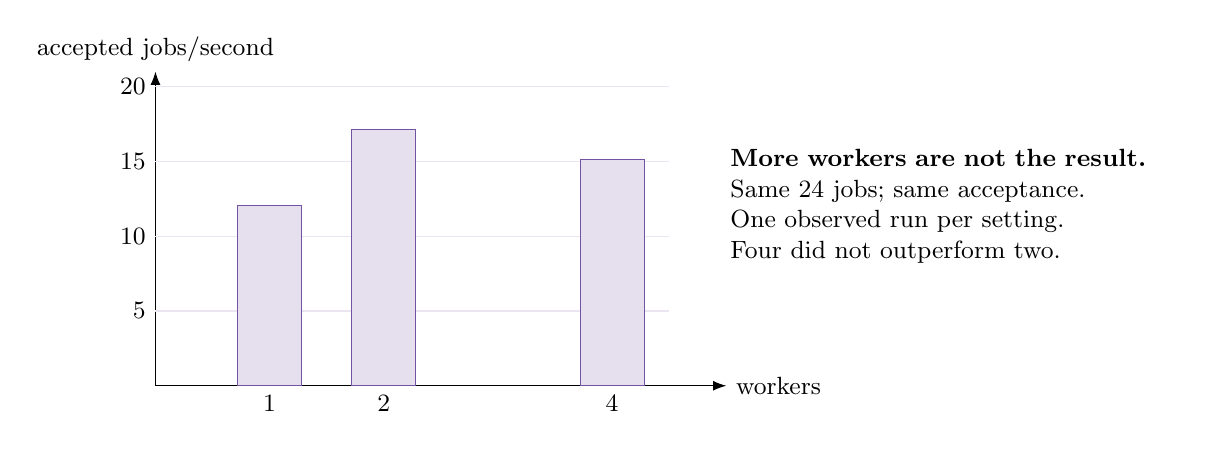
\begin{tikzpicture}[font=\small,>=Latex,x=1.45cm,y=.19cm]
\draw[->] (0,0)--(5,0) node[right]{workers};
\draw[->] (0,0)--(0,21) node[above,align=left]{accepted jobs/second};
\foreach \y in {5,10,15,20}{\draw[accent!15] (0,\y)--(4.5,\y);\node[left] at (0,\y){\y};}
\foreach \x/\y in {1/12.0546,2/17.1458,4/15.1424}{\draw[fill=accent!18,draw=accent] (\x-.28,0) rectangle (\x+.28,\y);\node[below] at (\x,0){\x};}
\node[align=left,text width=5.8cm,anchor=west] at (4.95,12) {\textbf{More workers are not the result.}\par Same 24 jobs; same acceptance.\par One observed run per setting.\par Four did not outperform two.};
\end{tikzpicture}
\caption{Measured local expansion. The source package also retains a separate capacity model; its schedule units are not mixed with this wall-clock measurement.}
\label{fig:scale}
\end{figure}

\subsection{What the launch kit cannot scale away}
For homogeneous work under a stable capacity model, let $e$ and $v$ be executor and validation time per accepted job, with $p$ executors and $q$ validators. If human review takes $h$ per job and available review time is $H$ per unit time, useful sustained throughput cannot exceed
\begin{equation}
 \lambda\le\min\{p/e,\ q/v,\ H/h,\ D\},
 \label{eq:capacity}
\end{equation}
where $D$ is actual arriving demand in the same time unit. This is resource accounting, not a discovered scaling law. Setup, retries, correlated faults, heterogeneous jobs and service deadlines need their own terms. In a separate illustrative schedule with one executor tick and three validator ticks per job, one validator caps throughput at one-third of a job per tick irrespective of whether there are one, two, four or eight executors. Those are model ticks, not observed seconds.

Diversification should run bounded experiments in parallel when resources permit. It need not wait for one buyer before exploring another offering. But each new mission receives a separate budget and explicit local authority; an asset copy does not duplicate funds or an acceptance right. Correlated verifier defects can scale with every copy. The present isolation is administrative and transactional on one trusted local host, not an adversarial multi-tenant sandbox.

\section{Failure handling is part of the release}
The companion rejects missing local authority, unsupported service families, invalid dimensions, out-of-scope workloads, stale source identities and insufficient reserved work. An incorrect result or revocation between execution and acceptance prevents acceptance. A replayed accepted request does not add another budget debit. Stop is cooperative at launch and commit boundaries; it does not preempt arbitrary code in the middle of an operation. The code only runs size-limited reviewed kernels.

A real subprocess is terminated immediately after it commits a work reservation. The pending attempt has no accepted output. Recovery refuses to clear a live worker; after the exited worker is confirmed absent, the local attempt is marked interrupted and its conservative reservation remains charged. A retry makes a separately charged attempt. This is deliberately honest about unmeasured partial work: it does not refund an interrupted attempt simply to make its budget look better. The independent checker verifies both attempt records.

The first concurrency development run exposed a SQLite disk-I/O failure. The implementation was corrected to close connections explicitly, configure write-ahead logging only during initialization and start worker processes with the spawn context. The failed log remains in the review record. Successful later runs do not erase it. These are local recovery checks, not distributed exactly-once payment semantics or production endurance evidence.

Known-good code and the zero-prefix profile remain available. Profile rollback also returns task implementations to the baseline. The shared profile never grants authority. A new version that passes the same finite predicates may still have an unknown defect; the actual request is independently checked on each delivery. A future externally exposed service additionally needs authenticated admission, per-client isolation, operational monitoring and explicit customer acceptance.

\section{A short path to an actual offering}
The commercial design is intentionally compact. Offer a bounded public-input report with an exact deliverable and an agreed check. Ask an actual beneficiary whether the reviewed result is worth the proposed price. Measure the operator's task interpretation and review time; neither is zero because a local script ran quickly. Price support, revalidation, unsuccessful proposals and maintenance where material. No fundraising, token issuance or new corporate structure is needed to test this proposition.

The decisive next deployment is an operator-run, independently selected public task for each promising offering. The owner approves its input, output contract and local budget. The operator records the delivery, review and beneficiary response. The next improvement experiment should use naturally occurring candidate changes, not only authored fault fixtures. Those tasks can run in parallel within the actual resource envelope. Broad RSI, marketplace and physical-infrastructure studies belong on a parallel research track, not as artificial gates before a useful local result.

\subsection{Four repositories; no four-dependency tax}
The source inspection on 22 October 2026 distinguishes preparation, candidate code, publication, installed qualification and live operation \cite{alignment,alphareadme,manager,jobs,fleet}. The local companion neither imports nor modifies the four repositories. It supplies a small integration target; its JSON records are \emph{not} asserted to match an existing production wire schema.

\begin{table}[htbp]\centering\small
\caption{Implementation bridge. These are intended mappings, not an executed four-repository integration or an activation authorization.}
\begin{tabularx}{\linewidth}{@{}P{3.2cm}YY@{}}\toprule
Surface & Role & Smallest handoff\\\midrule
AGI-Alpha-Agent-v0 & Orchestration, mission history, capability development & Map a local mission and review record to the qualified native schema; preserve source identity\\
AGIJobManager & Bounded commissioned work on the USDC route & Export a reviewed draft only; no posting or funding from this companion\\
AGIJobsv0 & Distinct \$AGIALPHA work/settlement route & Keep token, contract and admission identity separate; no automatic bridge\\
AGI-Fleet-Linux & Execution and separately authorized review & Package one reviewed local command for a qualified worker; preserve separate review authority\\\bottomrule
\end{tabularx}
\end{table}

The inspected Manager README calls production activation HOLD and separates software publication from intake activation. Fleet describes qualification prereleases and remaining physical/live-provider gates. Jobs distinguishes recorded paused deployments from commissioning. We do not turn those descriptions into a current chain-state claim. No address is copied into the companion; no wallet, chain query, signature, unpause or payment is required. The engineering handoff identifies the schema adapter and external operating qualification as remaining work, rather than calling this package an installed ecosystem release.

MONTREAL.AI's parent-ownership boundary remains unchanged. A service agreement creates no automatic equity or token-holder entitlement. USDC and \$AGIALPHA are distinct routes, not interchangeable measures of enterprise value. Any token-based service must justify its actual coordination burden; fewer unnecessary operations should not become a business-model failure \cite{economy}.

\section{Learn from stronger systems without waiting for them}
Test prioritization explicitly uses earlier execution information to detect failures sooner \cite{rothermel}; cost-sensitive variants warn that test counts and economic cost differ \cite{elbaum}. Counterexample-guided synthesis uses failed cases to constrain subsequent candidates \cite{cegis}. We do not claim to invent either idea. Our learner does not synthesize arbitrary programs: it changes the qualification itinerary of a reviewed finite candidate library and transfers that itinerary between typed offerings. A competent conventional engineer can implement it, and the expert-prefix result shows that a hand-built alternative can win.

AlphaEvolve develops executable algorithm candidates through model-driven search \cite{alphaevolve}. Darwin G\"odel Machine and MetaSkill-Evolve investigate agent or improvement-procedure modification at substantially different scales \cite{dgm,metaskill}. Vending-Bench evaluates extended operation in a simulated business \cite{vending}. Anthropic's long-running-agent harness work emphasizes preserved progress and explicit checks between sessions \cite{harness}. These are relevant ingredients and comparisons, not systems defeated by the present experiment. No provider or frontier model is evaluated here.

\subsection{Flint is a component option, not an inherited research organization}
Recursive's 21 October 2026 Flint release is a concrete contemporary signal \cite{flint,flintcard,flintcommit}. The first-party account attributes work across model development and inference to a small human-and-agent team using Eureka Machine. The released weights and the open \texttt{rec} inference engine do not constitute that complete research system. Developer-reported benchmark scores remain conditioned on their stated harnesses, sampling and hardware; this paper imports none as its own performance.

The model card marks the weights Apache-2.0 and supplies deployment-specific limitations. The inspected \texttt{rec} README targets specified Apple Silicon devices with at least 48 GB unified memory \cite{rec}. The present Linux CPU environment did not download or run Flint, and container network access was unavailable. Browser and connector access were sufficient for source review, not model execution. The launch kit therefore has no vendor dependency. An authorized team can later test a compatible current model as a proposal generator while keeping the same independent acceptance boundary. Acquiring weights does not establish access to the proprietary machinery that produced them.

\section{What can compound, and what remains a horizon}
The short-term asset is an executable launch path and a better tested method of improving it. The proposed commercial family can diversify into public numerical reports, performance investigations and dependency analyses. A useful expansion changes deliverables, beneficiaries or production methods; renaming another copy of the same job does not count as diversification.

Over a longer horizon, software can help construct instruments; instruments can enable discoveries; discoveries can qualify new manufacturing methods; useful production can finance energy and further productive infrastructure. Every transition requires actual evidence, rights, materials, capacity, operation and available cash. More agents do not create demand, eliminate heat, shorten every lead time or validate a new physical law. This paper establishes no exponential wealth trajectory or civilization-scale achievement.

The programme remains ambitious precisely because its first step is available. A field of many useful enterprises becomes more plausible when a verified common improvement lowers the burden of creating the next distinct offering. It becomes less plausible when every new idea first requires another platform or when bad variants are kept alive to inflate the count. Scale what proves useful, and retain the ability to stop.

\insight{\centering\textbf{ACTIVATE a growing diversity of useful enterprises.}\par
\textbf{EVOLVE the means that create them.}\par
\textbf{SCALE what proves useful.}\par\smallskip
Find your Alpha. Build your SUCCESSOR $\Omega$.}

\section{Conclusion and decisive tests}
The paper constructs a launchable local organization around existing capabilities, then uses operating failure evidence to change how a distinct offering's next improvement is evaluated. The acceptance contract is preserved; only the test itinerary changes. Its worst displacement is bounded, its favorable transfer is measured, its unsuccessful second update is rejected, and its concurrency limit is reported rather than hidden.

The strongest objection is also the next experiment: the candidate defects and task taxonomy are authored. A strong conventional ordering already beats the learned one on one offering. A useful external test must collect naturally occurring candidate changes and actual operator review costs on independently selected public tasks. Failure to reduce complete accepted-delivery cost, or disappearance of the transfer gain outside the authored taxonomy, would falsify the broader efficiency claim. None of that prevents a qualified baseline from delivering a bounded useful result today.

\noindent\textbf{Research status.} AI-assisted authoring and programming; deterministic local execution. No external service deployment, model-provider benchmark, paying customer, receipt, wallet action or production release occurred. Separate implementations share authorship and are not independent institutional reproduction. The original papers and repositories remain unchanged.

\clearpage
\appendix
\section{Run it, inspect it, change it}
The companion requires Python 3.11 or later with SQLite; the recorded tests use Python 3.13.5 on Linux. Process/recovery behavior is tested on that host. macOS portability is proposed, not installed-machine acceptance. No pip installation is required. From the extracted root:
\begin{lstlisting}
python code/launch.py init work
python code/launch.py activate work examples/range.json
python code/launch.py run work range-example
python code/launch.py inspect work
python code/launch.py tune work range-example --check-budget 512
python code/improve.py --trace work/range-example/improvement.json --out profile.json
python code/launch.py evolve work profile.json
python code/launch.py derive work range-example poly-example polynomial examples/polynomial_input.json --authorize-local
python code/launch.py tune work poly-example --seed 20261022 --check-budget 512
python code/launch.py run work poly-example
python code/launch.py stop work poly-example
python code/launch.py rollback work --version 0
\end{lstlisting}
The derived mission shares applicable machinery, not its parent's spending or permission history. The explicit command supplies a new local authorization and a separately recorded ceiling. The model is a trusted single-user workstation, not a credential service. Use the example JSON directly to set a different fresh ceiling.

A killed worker leaves an unfinished attempt and its reservation. After confirming that worker has exited:
\begin{lstlisting}
python code/launch.py recover work range-example
python code/launch.py run work range-example
\end{lstlisting}
Recovery refuses a process that may still be alive. It cannot authenticate a remote worker or solve distributed process identity. Repeated interruptions can exhaust the declared local budget; no unobserved work is refunded automatically.

\subsection{One-command research reproduction and separate checking}
\begin{lstlisting}
python code/study.py --out rerun
python code/check_results.py rerun
python -m unittest discover -s code -p 'test_*.py' -v
pdflatex -no-shell-escape -interaction=nonstopmode -halt-on-error -output-directory=paper paper/Autonomous_Enterprises_Activate_Evolve_Scale.tex
\end{lstlisting}
Repeat the TeX command to settle references. The driver refuses a nonempty result directory. The nine scientific and source-identity JSON files are deterministic; observed timings and environment metadata are saved separately in \texttt{timing.json}. The reproduction check excludes only that timing file and performs no normalization of scientific records. The source freeze and saved raw records make this distinction inspectable.

\section{Exact experiment design and accounting}
The source suite seed is 101; the next-cycle seed is 20261022. The source-derived profile is written before constructing continuation suites. The second profile consumes only the source and polynomial trace and is frozen before the reachability comparison. A 24-case confirmation uses seeds 20261122 through 20261145, alternating the two continuation families. These are author-chosen software checks, not external preregistration.

The cases enforce distinct service meanings. Range queries use $[l,r)$ and permit empty intervals. Polynomial multiplication returns the specified full coefficient length, including trailing zeros, and an empty vector when either input is empty. Reachability is directed and reflexive: an isolated source reaches itself. Two functions with similar output shapes cannot exchange these semantics. The independent oracles implement direct summation, coefficient-wise multiplication and Boolean transitive closure rather than importing the optimized implementations.

The candidate fixtures are deliberately disclosed. For example, dropping trailing polynomial zeros violates the full-length contract; omitting reflexive graph reachability violates an isolated-node request. The fixture set has no claim to approximate the frequency or diversity of real generated bugs. A broader generator can reveal different bottlenecks and reverse the learned ranking.

The recorded final execution has 37 passing unit-test methods. The saved-result checker validates 16,970 recorded candidate evaluations and 78 delivery records: six lifecycle deliveries plus the same 24-job workload in three concurrency settings. These overlapping counts are not independent enterprise replications. The interruption and wrong-result controls have separate records. An observed 6.287-second complete research driver is a single local measurement, not the total cost of writing, reviewing or deploying the system.

\subsection{Costs that are not free}
Runtime budgets charge explicit service and oracle counter increments. Improvement budgets charge candidate-test calls. Profile derivation scans trace rows; profile validation adds 90 calls. Version storage, database operations, hashing, serialization, memory, energy, review, taxes, support, customer acquisition and authoring are not all represented by those counters. Observed elapsed times include some local overhead but do not price it commercially. A real price must cover actual costs under actual accepted terms, not a conversion invented from operation counts.

For a paid offering with setup cost $K$, delivery cost $d$, review/help cost $h$, support provision $s$ and accepted price $p$, the elementary contribution condition after $N$ deliveries is $N(p-d-h-s)>K$. No value of $h$ or $s$ was measured here. A successful local command cannot establish this inequality, demand or cash timing. The price hypotheses in Table~\ref{tab:offers}'s discussion are therefore invitations to test, not financial recommendations.

\section{Evidence register and source custody}
\begin{longtable}{@{}P{3.1cm}P{5.3cm}P{6cm}@{}}\toprule
Claim & Actual evidence & Boundary\\\midrule\endhead
Three local offerings run & Three missions; six baseline/improved checked deliveries & Synthetic inputs; no external beneficiary acceptance\\
A shared profile changes later improvement work & Frozen profile causally passed to two later campaign evaluators & Authored finite defects; expert comparator wins one case\\
Acceptance is preserved & Predicate-permutation proof; 2,528 finite truth-vector checks & Pure deterministic tests; not universal program correctness\\
Unfavorable transfer has bounded overhead & Four-test control costs five rather than one & Weighted predicate costs required for a monetary bound\\
A second update is rejected & 90 versus 89 reachability checks; decisions equal & No multi-generation acceleration established\\
Budgets and authority remain separate & Transaction tests, revocation-before-commit, independent mission budgets & Trusted local host; no adversarial tenant isolation\\
Interrupted work remains accounted & Real subprocess exits with code 73 after reservation; separately charged retry & One injected interruption point; no external exactly-once claim\\
Bounded parallel activation works & 24 jobs accepted under 1, 2 and 4 workers & One timing per setting; extra processes are extra concurrency\\
An enterprise can earn revenue & Not established & Prices and beneficiaries hypothetical; no actual receipts\\
Broader RSI or industrial expansion & Research/deployment pathway & No learned model improvement or physical qualification\\\bottomrule
\end{longtable}

The selected predecessor is the supplied 23-page \emph{Build the Means of Building}, not the sibling \emph{Activate. Operate. Evolve.} manuscript. Its full supplied text was inspected; its PDF and TeX SHA-256 values match the requested identities. The TeX Git blob identity also matches the pinned repository result. Its historical code results are not claimed as newly rerun: this launch-focused assignment reuses their source/evidence distinction rather than repeating an unrelated suite.

\begin{lstlisting}
Predecessor commit:
f232d4cfa292484fc9a4ecae9f2d9d842101fcb5
PDF SHA-256:
a677bb4727f3af35038d1c972081f83bcc2e1019b65dea17da195c6eb078e7af
TeX SHA-256:
2d3481ebb3274f5f870cb3f445e6f6deca24ac6cd718ebd467186e40eb2fbc0d
TeX Git blob:
e0ba91b0de31b764ca568b1d903adb9a92f09f75
\end{lstlisting}

Relevant foundation and stage sections were inspected from supplied texts and the source excerpts retained in the conversation; not every stage paper was freshly read in full. The architectural manuscript's opening, evidence map and alignment document were inspected, not independently validated. The source audit records this scope. QUEBEC.AI's affiliation is supported by the supplied architectural author statement. Direct container downloads failed because network DNS was unavailable; accessible connected-repository and browser sources were used for the read-only inspection. That failure did not prevent the entirely local companion from running.

The Alpha main snapshot observed was \nolinkurl{0a668817284fed9010ad71ce405dbd5906ef2b28}. README and alignment blob identities for the four-repository map are retained in \texttt{provenance/Source\_Audit.md}. Release references in those documents are their maintainers' descriptions, not fresh downloaded-release, installed-runtime or live-chain acceptance. External primary-source inspection is dated 22 October 2026. It is a focused prior-art check, not an exhaustive priority claim.

\begin{thebibliography}{99}\small
\bibitem{predecessor} V. Boucher. \emph{Autonomous Enterprises: Build the Means of Building}. Supplied 23-page manuscript, 21 October 2026. Pinned source: \url{https://github.com/MontrealAI/AGI-Alpha-Agent-v0/blob/f232d4cfa292484fc9a4ecae9f2d9d842101fcb5/docs/Autonomous_Enterprises.pdf}.
\bibitem{ti} V. Boucher. \emph{Transformational Intelligence: Learning to Change the Game}. October 2026. Supplied foundation, selected sections inspected. \url{https://github.com/MontrealAI/AGI-Alpha-Agent-v0/blob/main/docs/Transformational_Intelligence.pdf}.
\bibitem{economy} V. Boucher. \emph{Invent the Economy: Transformational Intelligence for Creating Viable Markets}. October 2026. Supplied foundation, selected participation and finance sections inspected. \url{https://github.com/MontrealAI/AGI-Alpha-Agent-v0/blob/main/docs/Invent_the_Economy.pdf}.
\bibitem{alpha} V. Boucher. \emph{AGI ALPHA: A Scalable Substrate for Intelligence Organizations}. Pinned architectural manuscript, 30 April 2026. Opening and evidence architecture inspected. \url{https://github.com/MontrealAI/agialpha-first-real-loop/blob/bd920a6c52d820a087116bf59f2a4236d0494ac0/docs/manuscript/AGI_ALPHA_Unified_Publication_Final.md}.
\bibitem{rothermel} G. Rothermel, R. H. Untch, C. Chu and M. J. Harrold. Prioritizing Test Cases for Regression Testing. \emph{IEEE Transactions on Software Engineering}, 27(10):929--948, 2001. Author-hosted record inspected: \url{https://digitalcommons.unl.edu/csearticles/9/}. \url{https://doi.org/10.1109/32.962562}.
\bibitem{elbaum} S. Elbaum, A. G. Malishevsky and G. Rothermel. Incorporating Varying Test Costs and Fault Severities into Test Case Prioritization. \emph{ICSE}, 2001. Author-hosted abstract/record inspected: \url{https://digitalcommons.unl.edu/cseconfwork/135/}.
\bibitem{cegis} A. Solar-Lezama. \emph{Program Synthesis by Sketching}. UC Berkeley technical report UCB/EECS-2008-177, 2008. Author/institutional abstract and CEGIS lecture inspected. \url{https://www2.eecs.berkeley.edu/Pubs/TechRpts/2008/EECS-2008-177.html}; \url{https://people.csail.mit.edu/asolar/SynthesisCourse2020/Lecture10.htm}.
\bibitem{sqlite} SQLite. \emph{Transactions} and \emph{Write-Ahead Logging}. Official documentation, inspected 22 October 2026. \url{https://www.sqlite.org/lang_transaction.html}; \url{https://www.sqlite.org/wal.html}.
\bibitem{alignment} MONTREAL.AI. \emph{Alignment with the 198-page AGI ALPHA manuscript}. Source blob \nolinkurl{123a48a6454ed44f384b2560d8b1784ccd0ed387}, inspected 22 October 2026. \url{https://github.com/MontrealAI/AGI-Alpha-Agent-v0/blob/0a668817284fed9010ad71ce405dbd5906ef2b28/docs/agent/MANUSCRIPT_ALIGNMENT.md}.
\bibitem{alphareadme} MONTREAL.AI. \emph{AGI-Alpha-Agent-v0}, source snapshot \nolinkurl{0a668817284fed9010ad71ce405dbd5906ef2b28}, observed 22 October 2026. \url{https://github.com/MontrealAI/AGI-Alpha-Agent-v0}.
\bibitem{manager} MONTREAL.AI. \emph{AGIJobManager README}, lines 1--70 inspected, blob \nolinkurl{79264bda4b317b91feef9385fcf63296b39f55af}, 22 October 2026. \url{https://github.com/MontrealAI/AGIJobManager}.
\bibitem{jobs} MONTREAL.AI. \emph{AGIJobsv0 README}, lines 1--65 inspected, blob \nolinkurl{9d0d52e35f8798d9cd22c70ec2adb13e467a3379}, 22 October 2026. \url{https://github.com/MontrealAI/AGIJobsv0}.
\bibitem{fleet} MONTREAL.AI. \emph{AGI-Fleet-Linux README}, lines 1--85 inspected, blob \nolinkurl{1be7b329269d455488d1d72e902e8f32f23fdcc8}, 22 October 2026. \url{https://github.com/MontrealAI/AGI-Fleet-Linux}.
\bibitem{alphaevolve} A. Novikov et al. \emph{AlphaEvolve: A Coding Agent for Scientific and Algorithmic Discovery}. arXiv:2506.13131, 2025. Abstract inspected. \url{https://arxiv.org/abs/2506.13131}.
\bibitem{dgm} J. Zhang et al. \emph{Darwin G\"odel Machine: Open-Ended Evolution of Self-Improving Agents}. arXiv:2505.22954, 2025; revision 3, 12 March 2026. Abstract/record inspected. \url{https://arxiv.org/abs/2505.22954}.
\bibitem{metaskill} Z. Wang, M. Yan, J. Bi, S. Yan, V. Tresp and Y. Ma. \emph{MetaSkill-Evolve: Recursive Self-Improvement of LLM Agents via Two-Timescale Meta-Skill Evolution}. arXiv:2607.05297, 6 July 2026. Primary record/abstract inspected. \url{https://arxiv.org/abs/2607.05297}.
\bibitem{vending} A. Backlund and L. Petersson. \emph{Vending-Bench: A Benchmark for Long-Term Coherence of Autonomous Agents}. arXiv:2502.15840, 2025. Abstract inspected. \url{https://arxiv.org/abs/2502.15840}.
\bibitem{harness} Anthropic. \emph{Effective Harnesses for Long-Running Agents}. 26 November 2025. First-party engineering report, inspected 22 October 2026. \url{https://www.anthropic.com/research/effective-harnesses-for-long-running-agents}.
\bibitem{flint} Recursive. \emph{Introducing Flint}. Release announcement, October 2026; inspected 22 October. Developer account, not independently reproduced benchmarks. \url{https://recursive.com/updates/introducing-recursive-flint}.
\bibitem{flintcard} RecursiveSI. \emph{Flint model card}. Release specifications, limitations and Apache-2.0 label inspected 22 October 2026. \url{https://huggingface.co/RecursiveSI/flint}.
\bibitem{flintcommit} RecursiveSI. \emph{Flint commit history}: initial release, 21 October 2026, short identity \texttt{2a247be}. \url{https://huggingface.co/RecursiveSI/flint/commits/main}.
\bibitem{rec} Recursive. \emph{rec: local inference engine}. Hardware requirements and license label inspected 22 October 2026; not executed. \url{https://github.com/recursive-oss/rec}.
\end{thebibliography}
\end{document}
